% Fronteirs template Version 2.4 Generated 2014/03/12 %%%
\documentclass{frontiersSCNS} % for Science articles

%\setcitestyle{square}
\usepackage{url,lineno}
\linenumbers

\copyrightyear{}
\pubyear{}

\def\journal{Genetics}%%% write here for which journal %%%
\def\DOI{}
\def\articleType{Methods}
\def\keyFont{\fontsize{8}{11}\helveticabold }
\def\firstAuthorLast{Lawrence {et~al.}} %use et al only if is more than 1 author
\def\Authors{Travis J. Lawrence\,$^{1}$, Dana L. Carper\,$^{1}$, Katherine C.H. Amrine\,$^{1,2}$, Kyle Kauffman\,$^{3}$,Claudia Canales\,$^{3}$ and David H. Ardell\,$^{1,*}$}
% Affiliations should be keyed to the author's name with superscript numbers and be listed as follows: Laboratory, Institute, Department, Organization, City, State abbreviation (USA, Canada, Australia), and Country (without detailed address information such as city zip codes or street names).
% If one of the authors has a change of address, list the new address below the correspondence details using a superscript symbol and use the same symbol to indicate the author in the author list.
\def\Address{$^{1}$Quantitative and Systems Biology, University of California, Merced, CA, USA \\
$^{2}$Present address: Department of Viticulture and Enology, University of California, Davis, CA, USA \\ 
$^{3}$School of Natural Sciences, University of California, Merced, CA, USA}
% The Corresponding Author should be marked with an asterisk
% Provide the exact contact address (this time including street name and city zip code) and email of the corresponding author
\def\corrAuthor{David Ardell}
\def\corrAddress{Quantitative and Systems Biology, University of California, Merced, 5200 North Lake Road, Merced, CA , 95343, USA}
\def\corrEmail{dardell@ucmerced.edu}

% \color{FrontiersColor} Is the color used in the Journal name, in the title, and the names of the sections.

\begin{document}
\onecolumn
\firstpage{1}

\title[FAST]{FAST: Fast Analysis of Sequences Toolbox}
\author[\firstAuthorLast ]{\Authors}
\address{}
\correspondance{}
\topic{}% If your article is part of a Research Topic, please indicate here which.

\maketitle

\begin{abstract}

%%% Leave the Abstract empty if your article falls under any of the following categories: Editorial Book Review, Commentary, Field Grand Challenge, Opinion or specialty Grand Challenge.
\section{}
%As a primary goal, the abstract should render the general significance and conceptual advance of the work clearly accessible to a broad readership. References should not be cited in the abstract.Refer to \\ \url{http://www.frontiersin.org/}\texttt{\journal}\url{/authorguidelines} \\ or \textbf{Table\ref{Tab:01}} for abstract requirement and length according to article type.


\tiny
 \keyFont{ \section{Keywords:} Text Text Text Text Text Text Text Text } %All article types: you may provide up to 8 keywords; at least 5 are mandatory.
\end{abstract}

\section{Introduction}

% For Original Research Articles, Clinical Trial Articles, and Technology Reports the introduction should be succinct, with no subheadings.
%
% For Clinical Case Studies the Introduction should include symptoms at presentation, physical exams and lab results.
%
The field of molecular biology has changed significantly with the
advent of next generation sequencing technology. It is now commonplace
to analyze gigabases worth of data per experiment. Traditionally
programs were developed for visualization and for basic sequence
manipulation by a GUI interface \citep{Smith1994, Rampp2006}. Most
available bioinformatic toolkits are designed for specific types of
data or analysis requiring several toolkits to be installed. Moreover,
each toolkit often requires a different file format making data
analysis difficult.

The FAST utilities are modeled after the
standard Unix toolkit\citep{Peek2001}, follow the Unix philosophy of
``do one thing and do it well'' \citep{Stutz2000}, and are written in
PERL using bioperl packages \citep{Stajich2002}. This makes FAST
utilities easy to adopt if you are familiar with the Unix toolkit and
allows fast sequence analysis even on large datasets. FAST utilities
have a uniform interface requiring FASTA formatted files and are
capable of reading data from STDIN. This allows quick prototyping of
sequence analysis problems by piping data between several
utilities. Additionally, fasconvert can convert to/from fasta from/to
several formats increasing the flexibility and usability of
FAST. Extensive documentation has been developed for each utility
along with useful error messages following the recommendations of
\cite{Seemann2013} to increase usability. Lastly, FAST is open source,
which makes it available to anyone free of cost. This is in line with
the call to make science more assessable, open, and reproducible by
other scientists and the public \citep{Groves2012}.  

FAST is split
into three categories selection, transformation, and annotation and
analysis. The selection category contains utilities designed to select
sequences and sites from alignments based on several different
criteria. For example fasgrep selects sequences by matching a regular
expression to the ID, description, or sequence. The transformation
utilities are used to modify the ID, description, sequence, or order
of sequences using several criteria. For example, fastaxsort sorts
sequences within a multifasta file based on NCBI taxonomy
\citep{Benson2009, Sayers2009}. The annotation and analysis category
contains utilities to calculate sequence composition, codon usage,
sequence length, and basic population genetic statistics. Additionally
these utilities can also append the results of the analysis to the
sequence description, which then can be used as selection criteria by
the utilities in the selection category.

Some utilities within FAST
have overlapping function with those found within other toolkits. For
example sequence composition, sequence translation, and codon usage
are available in the EMBOSS package \citep{Rice2000}. Another example
is the Bioinformatics Toolbox \citep{White2014} that has utilities to
select only unique sequences and extract sequences from Genbank files
based on gene name, which have overlapping function with fasuniq and
gbfeat2fas respectively. However, the utilities in EMBOSS
\citep{Rice2000} and Bioinformatics Toolbox \citep{White2014} lack a
uniform interface, are not modeled after the Unix toolkit, and do not
have the ability to use regular expressions to select and manipulate
sequences. However, FAST also contains several utilities that have
unique functionality. For example gbalncut takes a multiple sequence
alignment annotated with a genomic feature and a genbank file and
allows you to select certain regions of the alignment such as all the
exons or the coding sequence. Another example is fastaxsort that
allows sorting of a multifasta file based on NCBI taxonomy
\citep{Benson2009, Sayers2009}.

%\begin{methods}
\section{Description}

Learnability of the FAST tools is helped by making interface
components such as specific options, consistent with the standard UNIX
tools amd across the FAST suite. Learning one FAST tool generally
helps the user anticipate how to use others. In addition,
specification of numerical ranges, regular expressions and other
useful parameters follows standard Perl and UNIX conventions, all with
the intent of making the tools fast and easy to learn.

FAST is compatible with the zero-based indexing if the sequence
identifier is thought as the zero^th field of the identifier
line. This field must exist in Data selection in FAST is
one-based as is conventional BioPerl coordinates and bioinformatics
generally.

\subsection{Selection Utilities}

\subsection{Transformation Utilities}


\subsection{Annotation and Analysis Utilities}
\subsection{Usability and Scalability}

%\end{methods}

\section{Discussion}

Text Text Text Text Text Text  Text Text Text Text Text Text Text Text Text  Text Text Text Text Text Text Text Text Text Text.
Additional Requirements:
\subsection{Data Sharing}

Frontiers supports the policy of data sharing, and authors are advised to make freely available any materials and information described in their article, and any data relevant to the article (while not compromising confidentiality in the context of human-subject research) that may be reasonably requested by others for the purpose of academic and non-commercial research. In regards to deposition of data and data sharing through databases, Frontiers urges authors to comply with the current best practices within their discipline.

\section*{Disclosure/Conflict-of-Interest Statement}
%Frontiers follows the recommendations by the International Committee of Medical Journal Editors (http://www.icmje.org/ethical_4conflicts.html) which require that all financial, commercial or other relationships that might be perceived by the academic community as representing a potential conflict of interest must be disclosed. If no such relationship exists, authors will be asked to declare that the research was conducted in the absence of any commercial or financial relationships that could be construed as a potential conflict of interest. When disclosing the potential conflict of interest, the authors need to address the following points:
%•	Did you or your institution at any time receive payment or services from a third party for any aspect of the submitted work?
%•	Please declare financial relationships with entities that could be perceived to influence, or that give the appearance of potentially influencing, what you wrote in the submitted work.
%•	Please declare patents and copyrights, whether pending, issued, licensed and/or receiving royalties relevant to the work.
%•	Please state other relationships or activities that readers could perceive to have influenced, or that give the appearance of potentially influencing, what you wrote in the submitted work.

The authors declare that the research was conducted in the absence of any commercial or financial relationships that could be construed as a potential conflict of interest.

\section*{Author Contributions}
%When determining authorship the following criteria should be observed:
%•	Substantial contributions to the conception or design of the work; or the acquisition, analysis, or interpretation of data for the work; AND
%•	Drafting the work or revising it critically for important intellectual content; AND
%•	Final approval of the version to be published ; AND
%•	Agreement to be accountable for all aspects of the work in ensuring that questions related to the accuracy or integrity of any part of the work are appropriately investigated and resolved.
%Contributors who meet fewer than all 4 of the above criteria for authorship should not be listed as authors, but they should be acknowledged. (http://www.icmje.org/roles_a.html)

The statement about the authors and contributors can be up to several sentences long, describing the tasks of individual authors referred to by their initials and should be included at the end of the manuscript before the References section.


\section*{Acknowledgement}
We acknowledge NSF, Professsors Laura Landweber, Siv Andersson and
Leif Kirsebom, the Linnaeus Centre for Bioinformatics and Biomedical
Computing group, the Graduate Research Council and Chancellor's award
 to DHA. of UC Merced

\paragraph{Funding\textcolon} Text Text Text Text Text Text  Text Text.

\section*{Supplemental Data}
Text Text Text Text Text Text  Text Text Text Text Text Text Text Text Text  Text Text Text Text Text Text Text Text Text  Text Text Text.

\bibliographystyle{frontiersinSCNS&ENG} % for Science and Engineering articles
%\bibliographystyle{frontiersinHLTH&FPHY} % for Health and Physics articles
\bibliography{FAST}

\section*{Figures}

%%% Use this if adding the figures directly in the mansucript, if so, please remember to also upload the files when submitting your article
%%% There is no need for adding the file termination, as long as you indicate where the file is saved. In the examples below the files (logo1.jpg and logo2.eps) are in the Frontiers LaTeX folder
%%% If using *.tif files convert them to .jpg or .png

\begin{figure}
\begin{center}
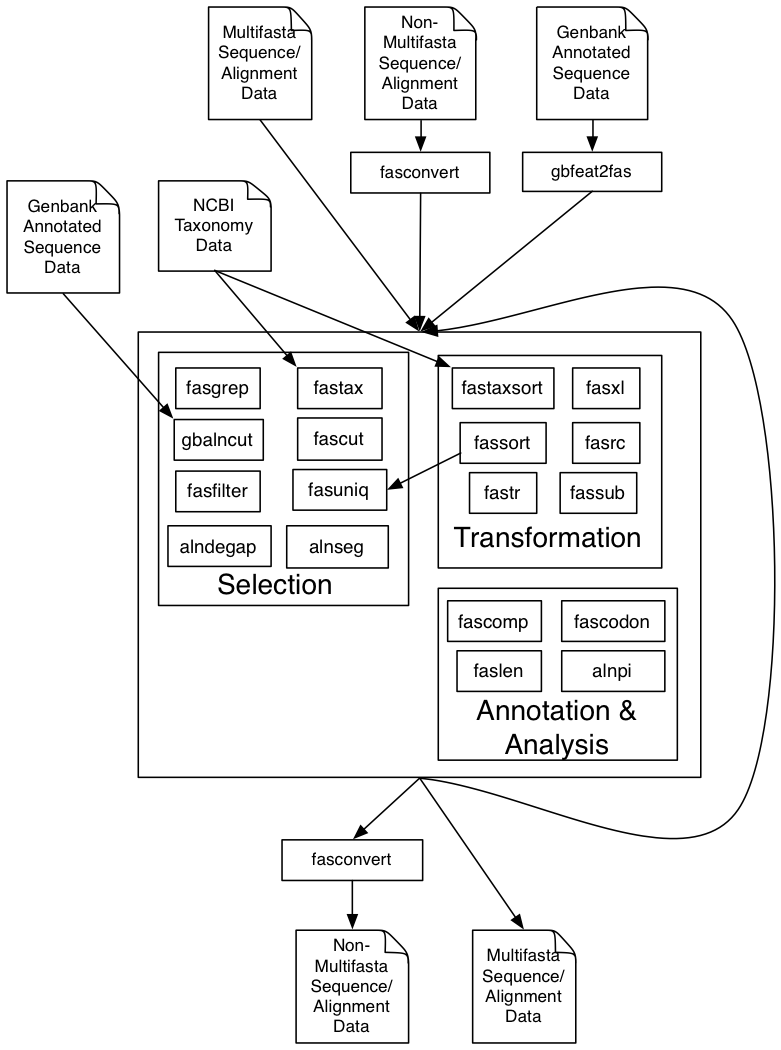
\includegraphics[width=3.5cm]{FAST_v2}% This is a *.jpg file
\end{center}
 \textbf{\refstepcounter{figure}\label{fig:01} Figure \arabic{figure}.}{ Enter the caption for your figure here.  Repeat as  necessary for each of your figures }
\end{figure}

%\begin{figure}
%\begin{center}
%
\includegraphics[width=3.5cm]{logo2}% This is an *.eps file
%\end{center}
% \textbf{\refstepcounter{figure}\label{fig:02} Figure \arabic{figure}.}{ Enter the caption for your figure here.  Repeat as  necessary for each of your figures }
%\end{figure}

 \textbf{Figure 1.}{ Enter the caption for your figure here.  Repeat as  necessary for each of your figures.}\label{fig:01}% If you don't add the figures in the LaTeX files, please upload them when submitting the article.

%%% Frontiers will add the figures at the end of the provisional pdf automatically %%%

%%% The use of LaTeX coding to draw Diagrams/Figures/Structures should be avoided. They should be external callouts including graphics.

\end{document}
